% Sección del artículo — dueño: P5. Sólo el dueño edita este archivo (v18).
\subsection{Arquitectura propuesta}
\textbf{Módulo mosca.} Cada cuadro del ojo $x_\tau\in\{0,1\}^{32\times32}$ pasa por un
codificador convolucional compartido $\phi$ (tres bloques conv$3\times3$--BN--ReLU--MaxPool
con 16, 32 y 64 filtros, y una capa lineal a 128 dimensiones). Una GRU~\cite{cho2014}
integra la secuencia de los últimos $T=4$ cuadros,
\begin{equation}
h_\tau = \mathrm{GRU}\big(\phi(x_\tau), h_{\tau-1}\big),\qquad \tau = t-T+1,\dots,t,
\end{equation}
y la decisión se toma con el último estado y el objetivo relativo codificado $g_t$:
$p_\theta(a\mid x_{t-T+1:t}, g_t) = \mathrm{softmax}\big(f([h_t; \psi(g_t)])\big)$.
Como comparación se usan un MLP (\nfbParamsMLP{} parámetros) y una CNN de un solo cuadro
(\nfbParamsCNN{}), y una variante con un codificador Transformer~\cite{vaswani2017}
(\nfbParamsTransformer{}) en lugar de la GRU; la propuesta CNN+GRU tiene \nfbParamsGRU{}
parámetros (Fig.~\ref{fig:redesmosca}).

\begin{figure*}[t]
\centering
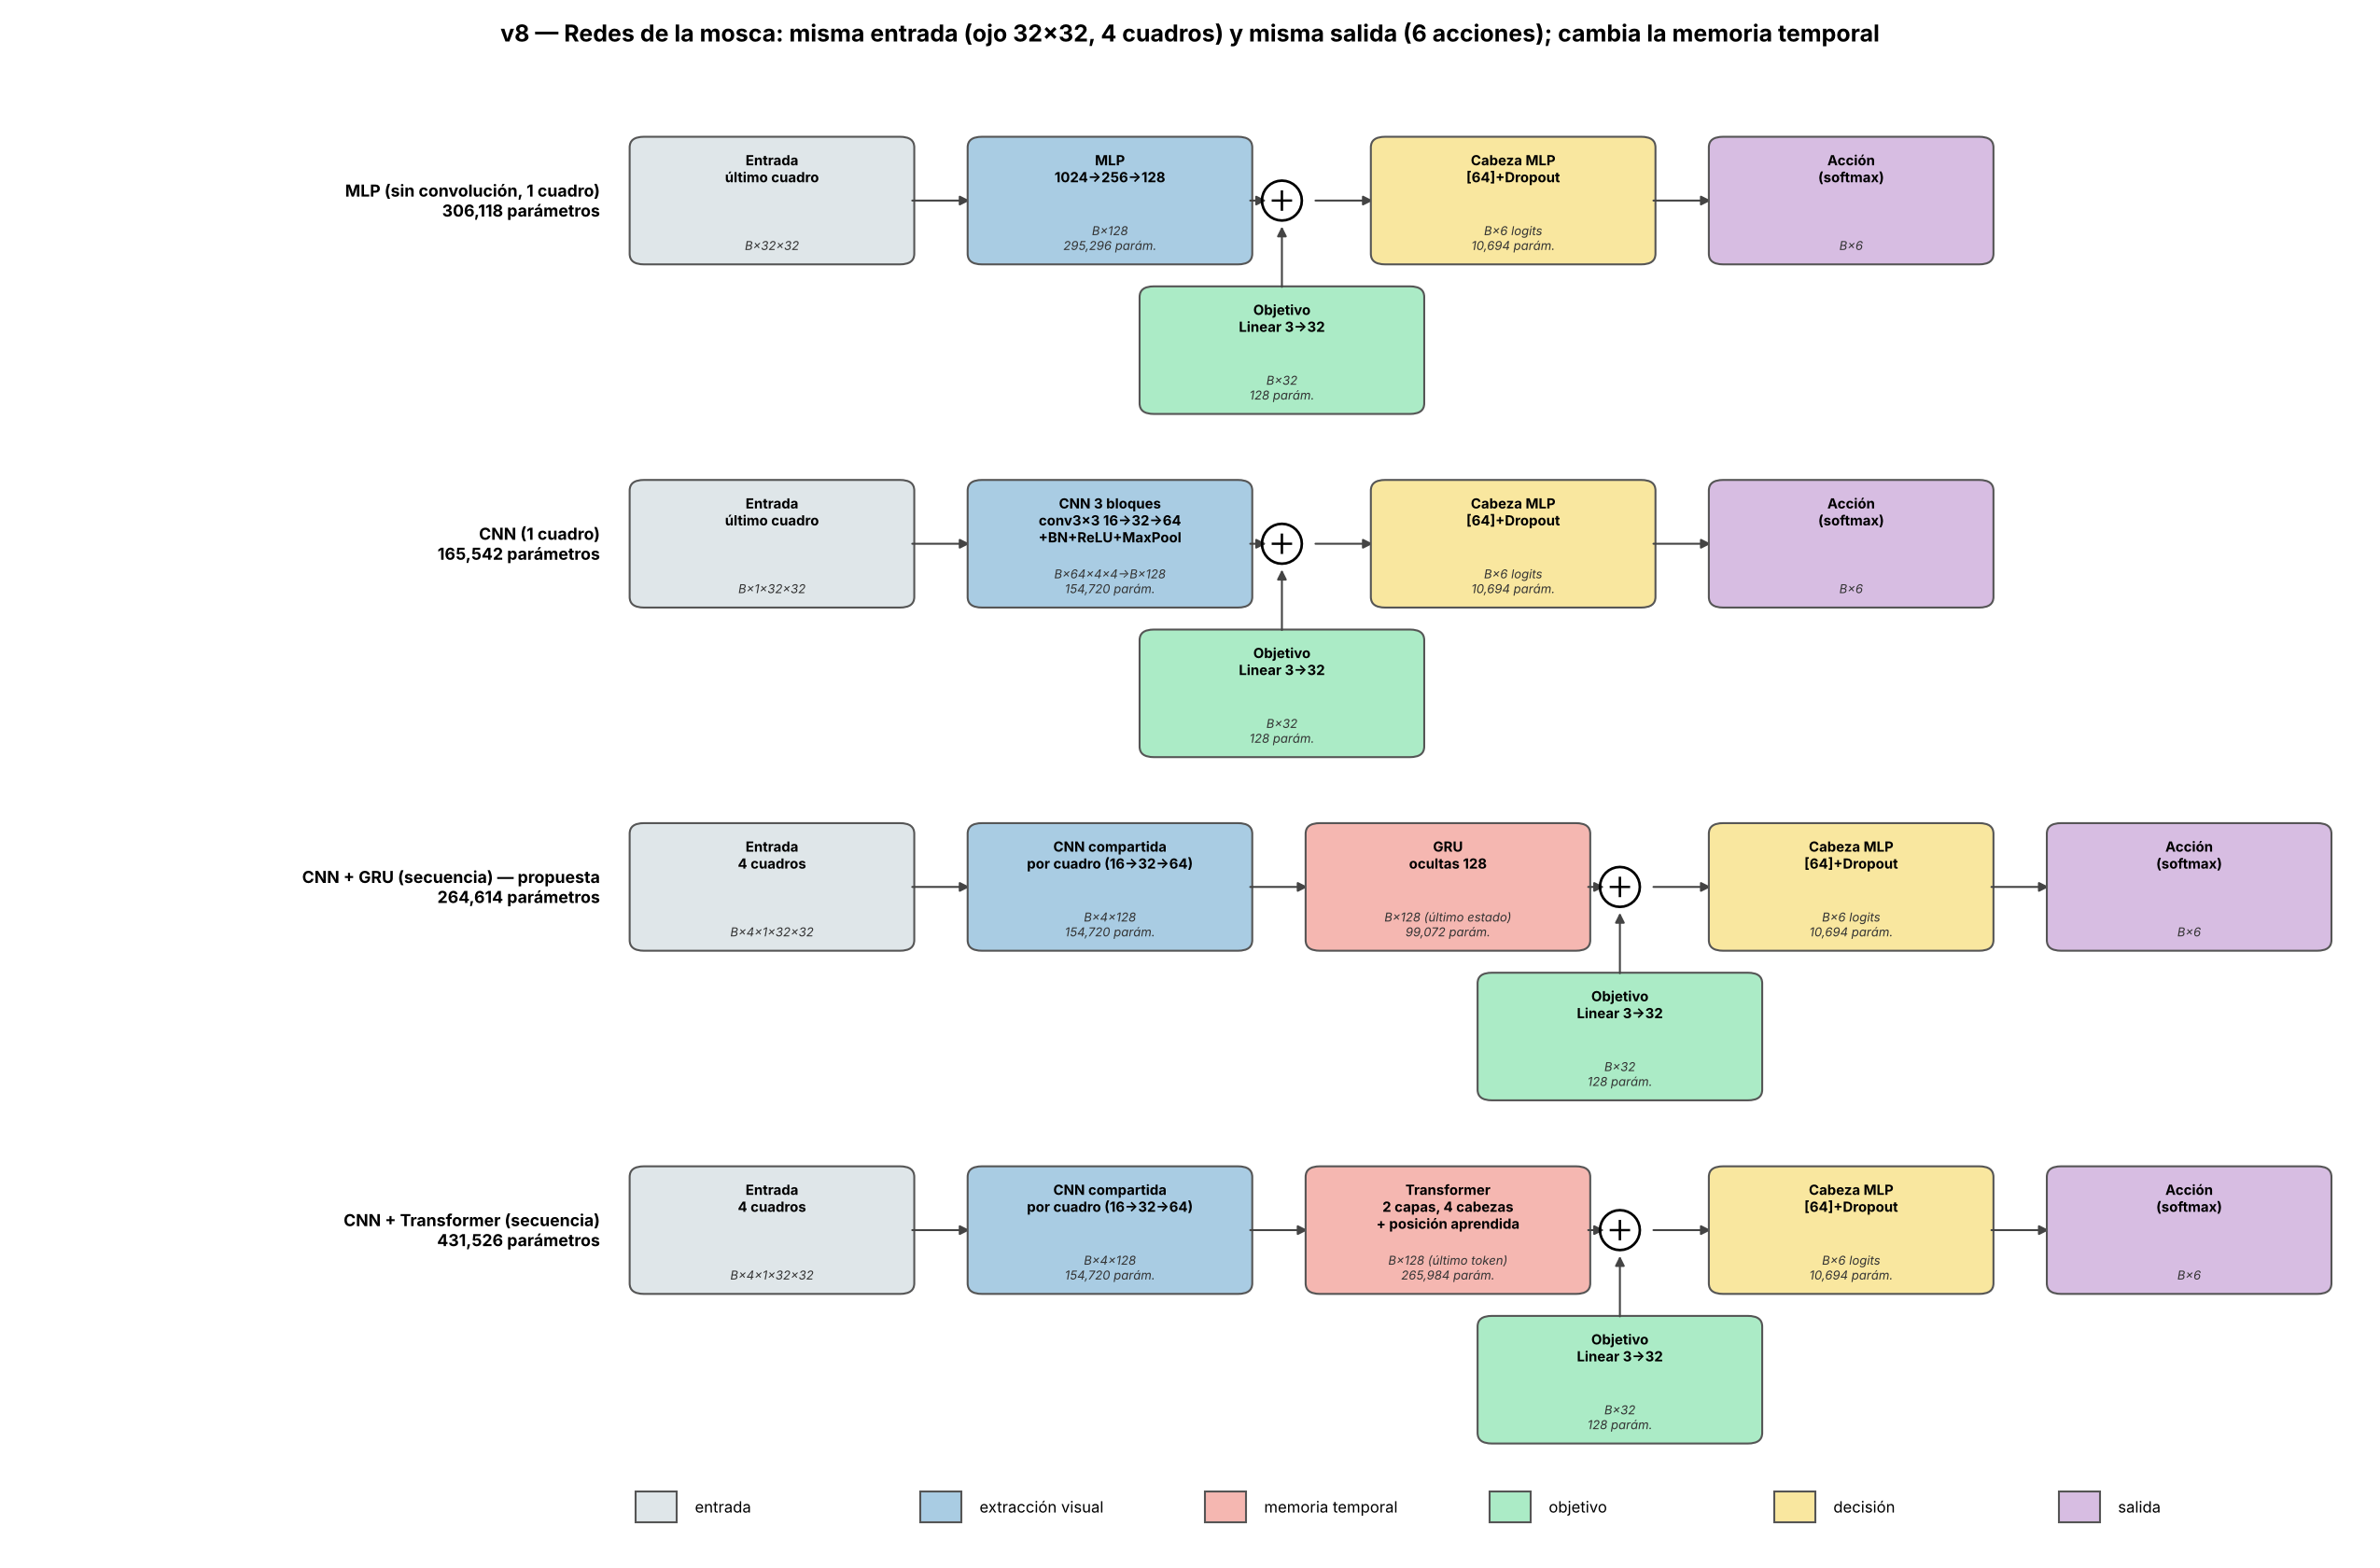
\includegraphics[width=0.95\textwidth]{v8_redes_mosca}
\caption{Redes del módulo mosca: misma entrada y salida; cambia la memoria temporal.}
\label{fig:redesmosca}
\end{figure*}

\textbf{Módulo abeja.} Inspirado en el modelo de instantáneas de las abejas~\cite{cartwright1983},
el dron memoriza al despegar la silueta panorámica de la base $s_0\in[0,1]^{72}$, alineada
con la brújula. Una red siamesa 1D $\rho$ con relleno circular codifica la vista actual $s_t$
y la memorizada; la cabeza recibe $[\rho(s_t);\rho(s_0);\rho(s_t)-\rho(s_0)]$ y predice
$(\cos\hat\theta,\sin\hat\theta,\log(1+\hat d))$, la dirección y la distancia a la base.
Se entrena minimizando
\begin{equation}
\begin{split}
\mathcal{L}_{\text{abeja}} ={}& \big(1-\cos(\hat\theta-\theta)\big)\\
&+ \lambda\,\mathrm{SmoothL1}\big(\log(1+\hat d),\log(1+d)\big),\quad \lambda=0.5.
\end{split}
\label{eq:abeja}
\end{equation}
La cabeza aplana el mapa de rasgos ($64\times18$) y lo pasa por un MLP con
\emph{dropout} de 0.1; concentra 148\,000 de los 172\,547 parámetros. Para la ablación se
definen tres variantes que cambian una sola decisión: sólo la vista actual, sin la resta
$\rho(s_t)-\rho(s_0)$, y una \emph{lectura vectorial} compacta en la que cada uno de los 18
sectores (centro $\varphi_k$) emite un voto $w_k$ y la dirección es
$\hat{\mathbf v}=\sum_k w_k(\cos\varphi_k,\sin\varphi_k)$, como el ALV pero con pesos
aprendidos (\nfbParamsAbejaCompacta{} parámetros en total).
La línea base es el vector promedio de hitos (ALV)~\cite{lambrinos2000}, que con las mismas
entradas obtiene un error angular mediano de \nfbAlvErrorMediano{} en validación (Fig.~\ref{fig:abeja}).

\begin{figure*}[t]
\centering
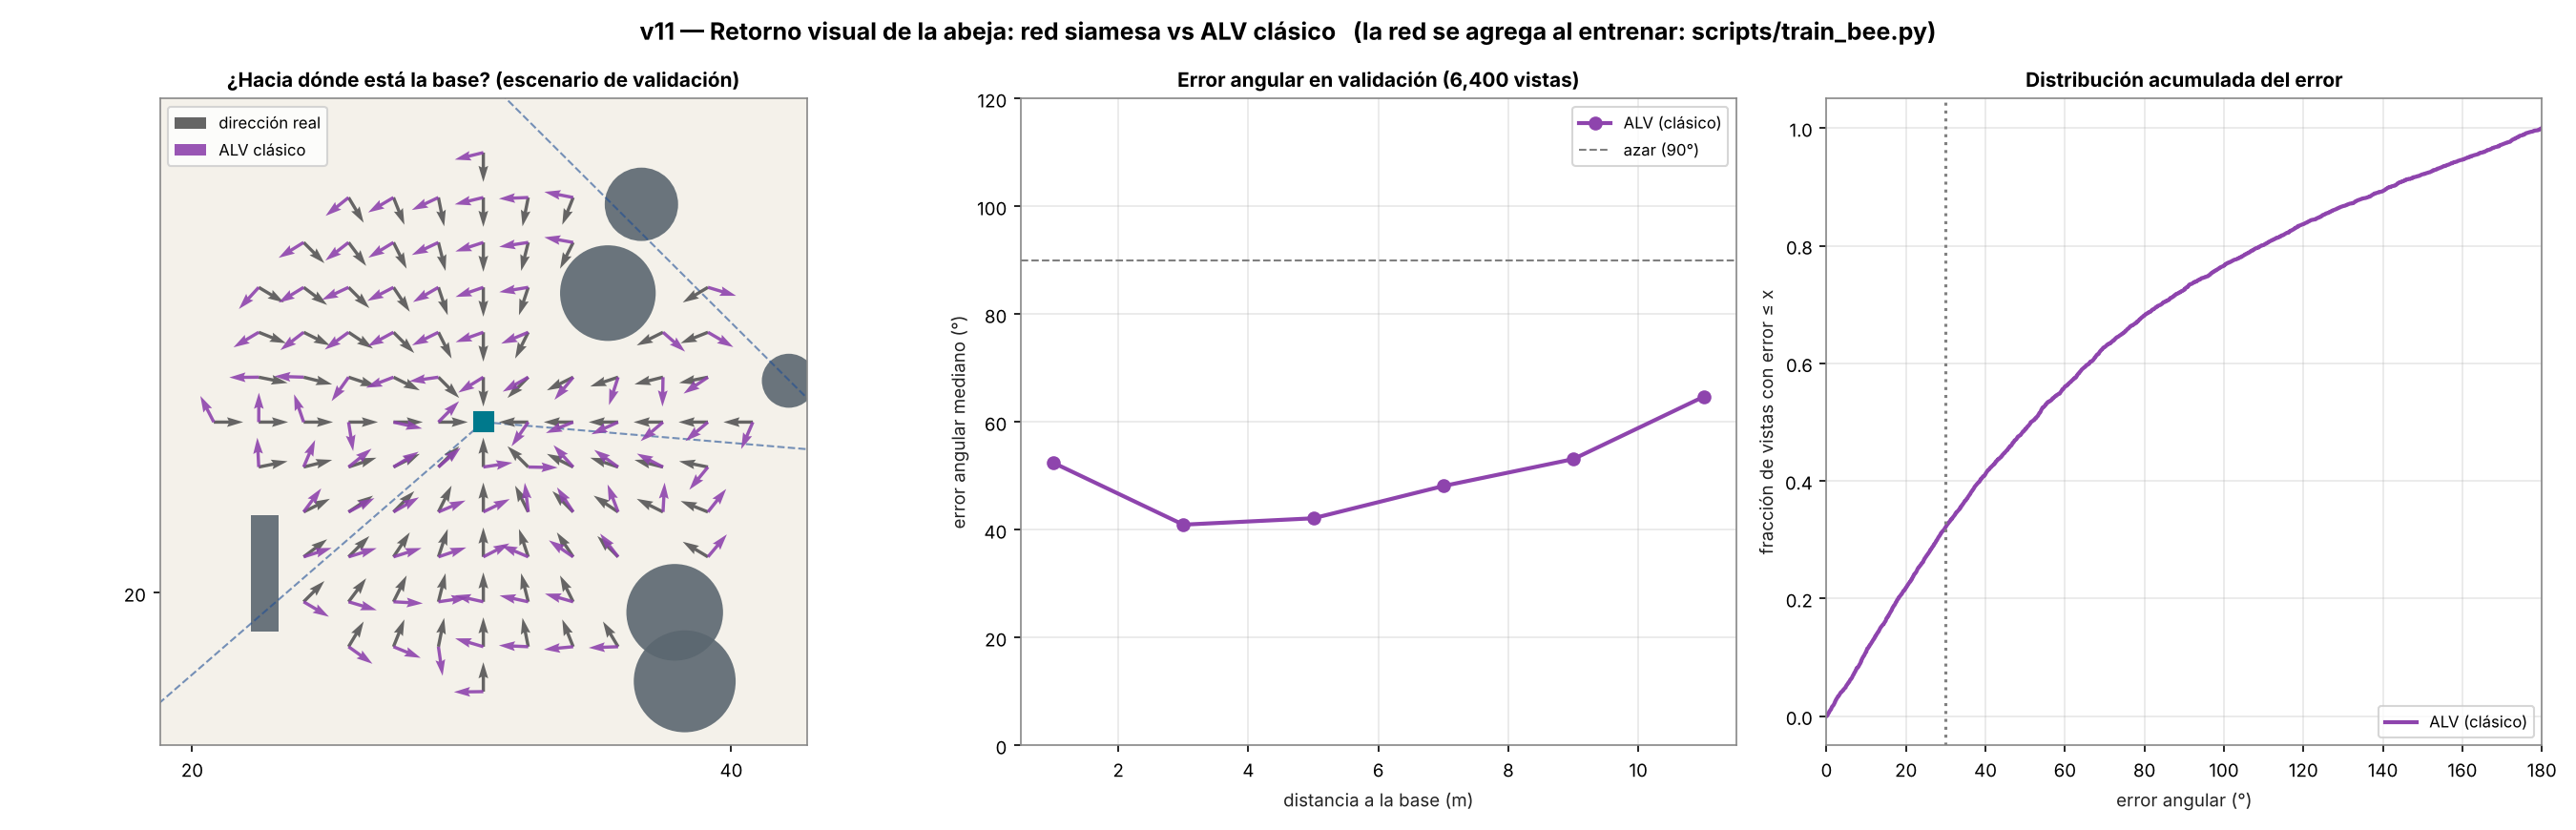
\includegraphics[width=0.95\textwidth]{v11_retorno_abeja}
\caption{Retorno visual: dirección real, ALV clásico y red de la abeja (validación).}
\label{fig:abeja}
\end{figure*}

\textbf{Integración y seguridad.} La abeja actúa como navegador de alto nivel (memoria
de la ruta, fase de la misión y, sin GPS, retorno visual), la mosca como control local y un
supervisor independiente de las redes veta, usando sólo el anillo de distancias, las
maniobras cuya posición prevista quede a menos de $r+0.6$\,m de un obstáculo detectado
(Fig.~\ref{fig:hibrido}). Con el controlador directo, el supervisor reduce los choques con
obstáculos fijos de \nfbChoquesDirectoFijos{} a \nfbChoquesDirectoSupFijos{}, pero no evita
los choques con obstáculos móviles, que llegan desde fuera del alcance de los rayos.

\begin{figure*}[t]
\centering
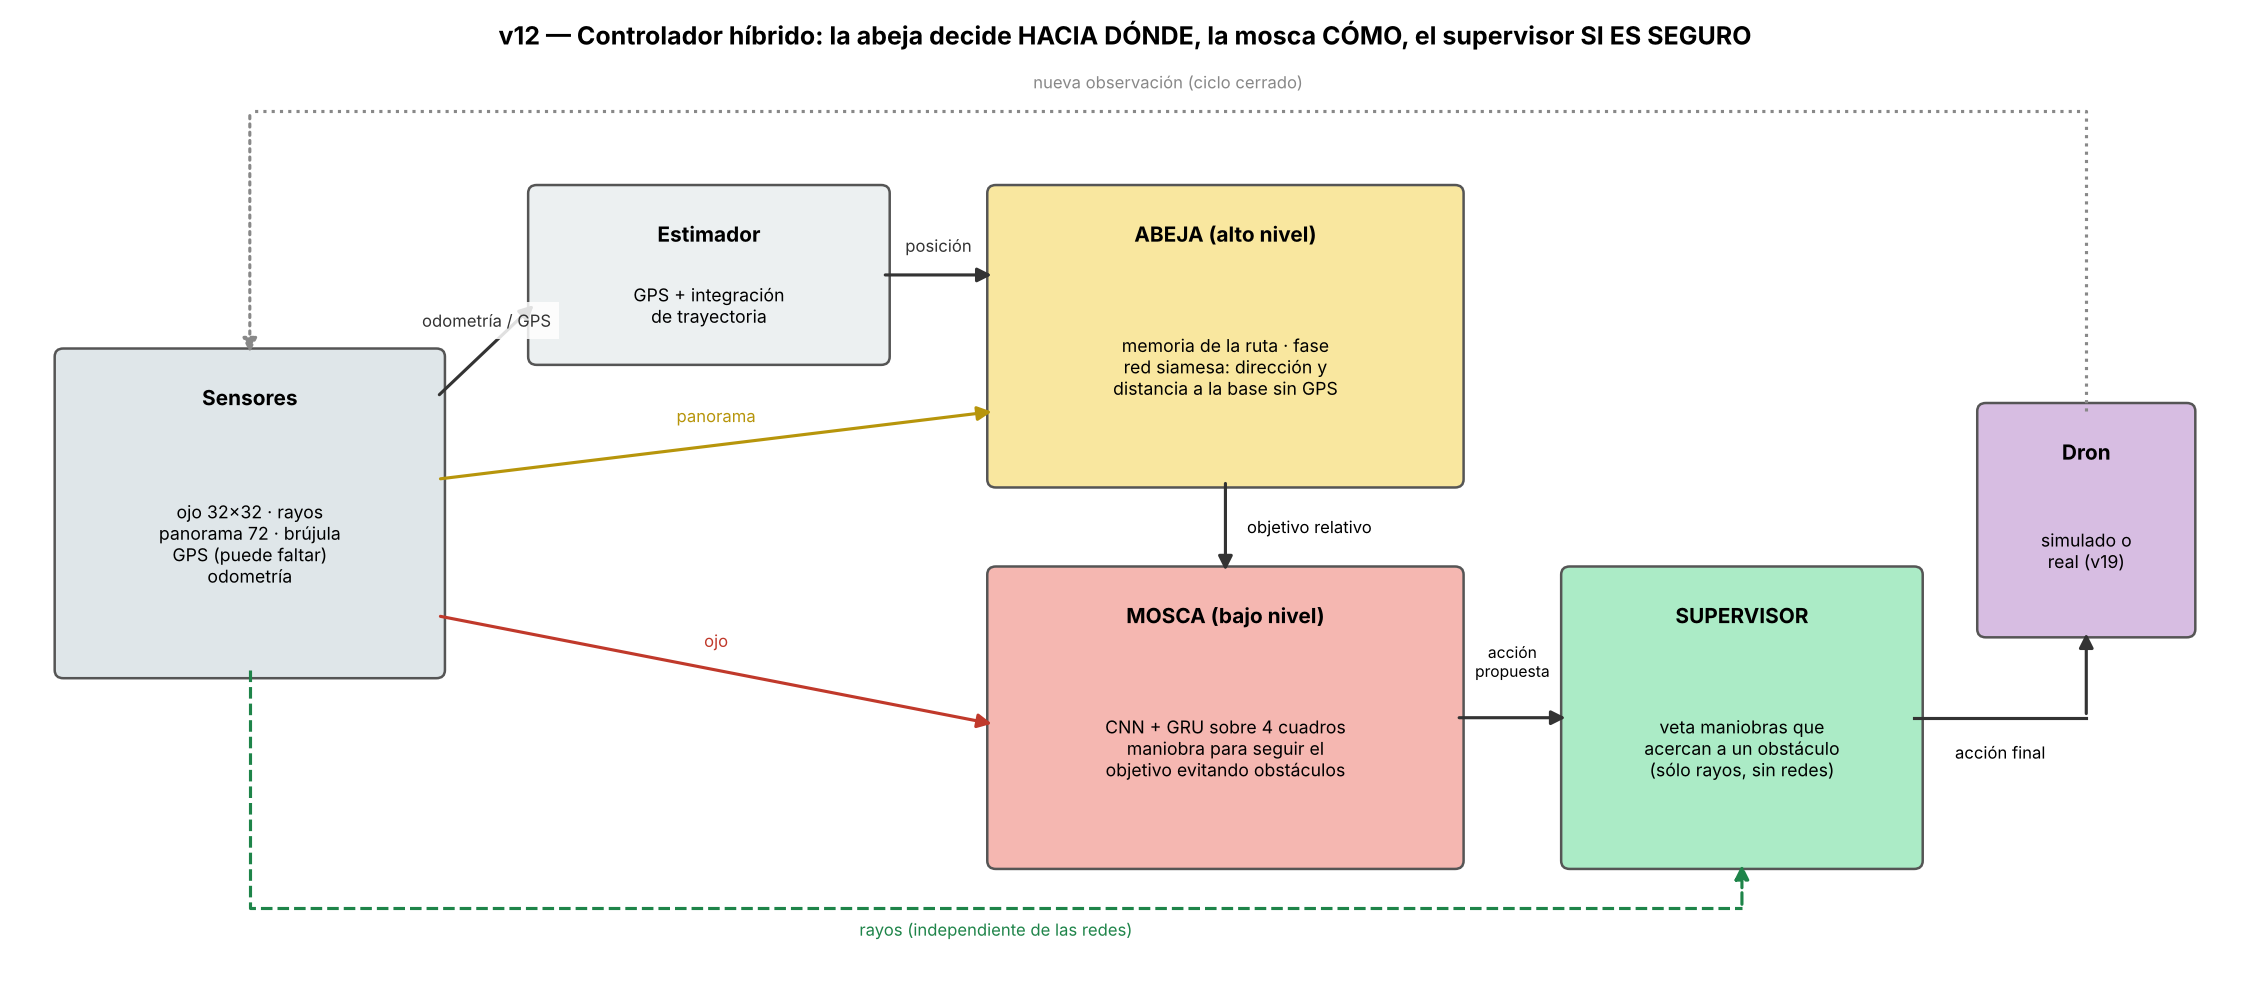
\includegraphics[width=0.9\textwidth]{v12_arquitectura_hibrida}
\caption{Controlador híbrido: abeja (hacia dónde), mosca (cómo) y supervisor (si es seguro).}
\label{fig:hibrido}
\end{figure*}
